\chapter{System design}
\label{chap:System design}
%Hvad dette chapter skal indeholde:
%Hvordan positionen på robotten bliver udregnet og evt hvordan den skal kunne bevæge sig?????(referer og citer hvad vi har skrevet i incerement two)
%Hvordan vi skal have Kinect og Arduino til at snakke sammen(Program i kinect der sender data til wifishield som arduinoet kan bruge)
%Skal vi have noget med afgrænsningen til at vi bouncer med her????
%Hvordan vores schedule skal fungere? Teorien bag det også kan det blive forklaret i implementationen.
%I system design skal vi også snakke om memory management evt ?? 
%Skal vi skirve om den billede analyse som kinecten laver??

\section{Software choices}
\label{sec:Software choices}
%Hviket software vi bruger til at udvikle robotten og hvilke libraries vi bruger? SKal vi evt. have en section om Hardware choices? Skal vi skrive her at vi bruger Arduino's ide og at vi bruger 1.0.3??
\subsection{Arduino IDE}
\label{sec:Arduino IDE}
After testing the Arduino IDE 1.6.12 with the code defined on the Arduino website's Wifi-guide \citep{wg}, it was discovered that the Wifi library was not compatible in the IDE in a series of newer versions. The library was supported in version 1.0.3, which is why this particular IDE version is used in this project. The newer IDE's has increased security, which would actively refuse any TCP connection from the computer.

\section{Robot design}
\label{sec:Robot design}
%Kort om hvordan vi har lavet robotten? Vi kan evt. have noget med hvordan vi placere vores kinect i en subsection?
The purpose of the robot is to catch the thrown object, by driving to the impact point of the object and the ground within the predefined area. The final design of the robot is shown in figure \ref{robot}.

\begin{figure}[h]
	\centering
	\fbox{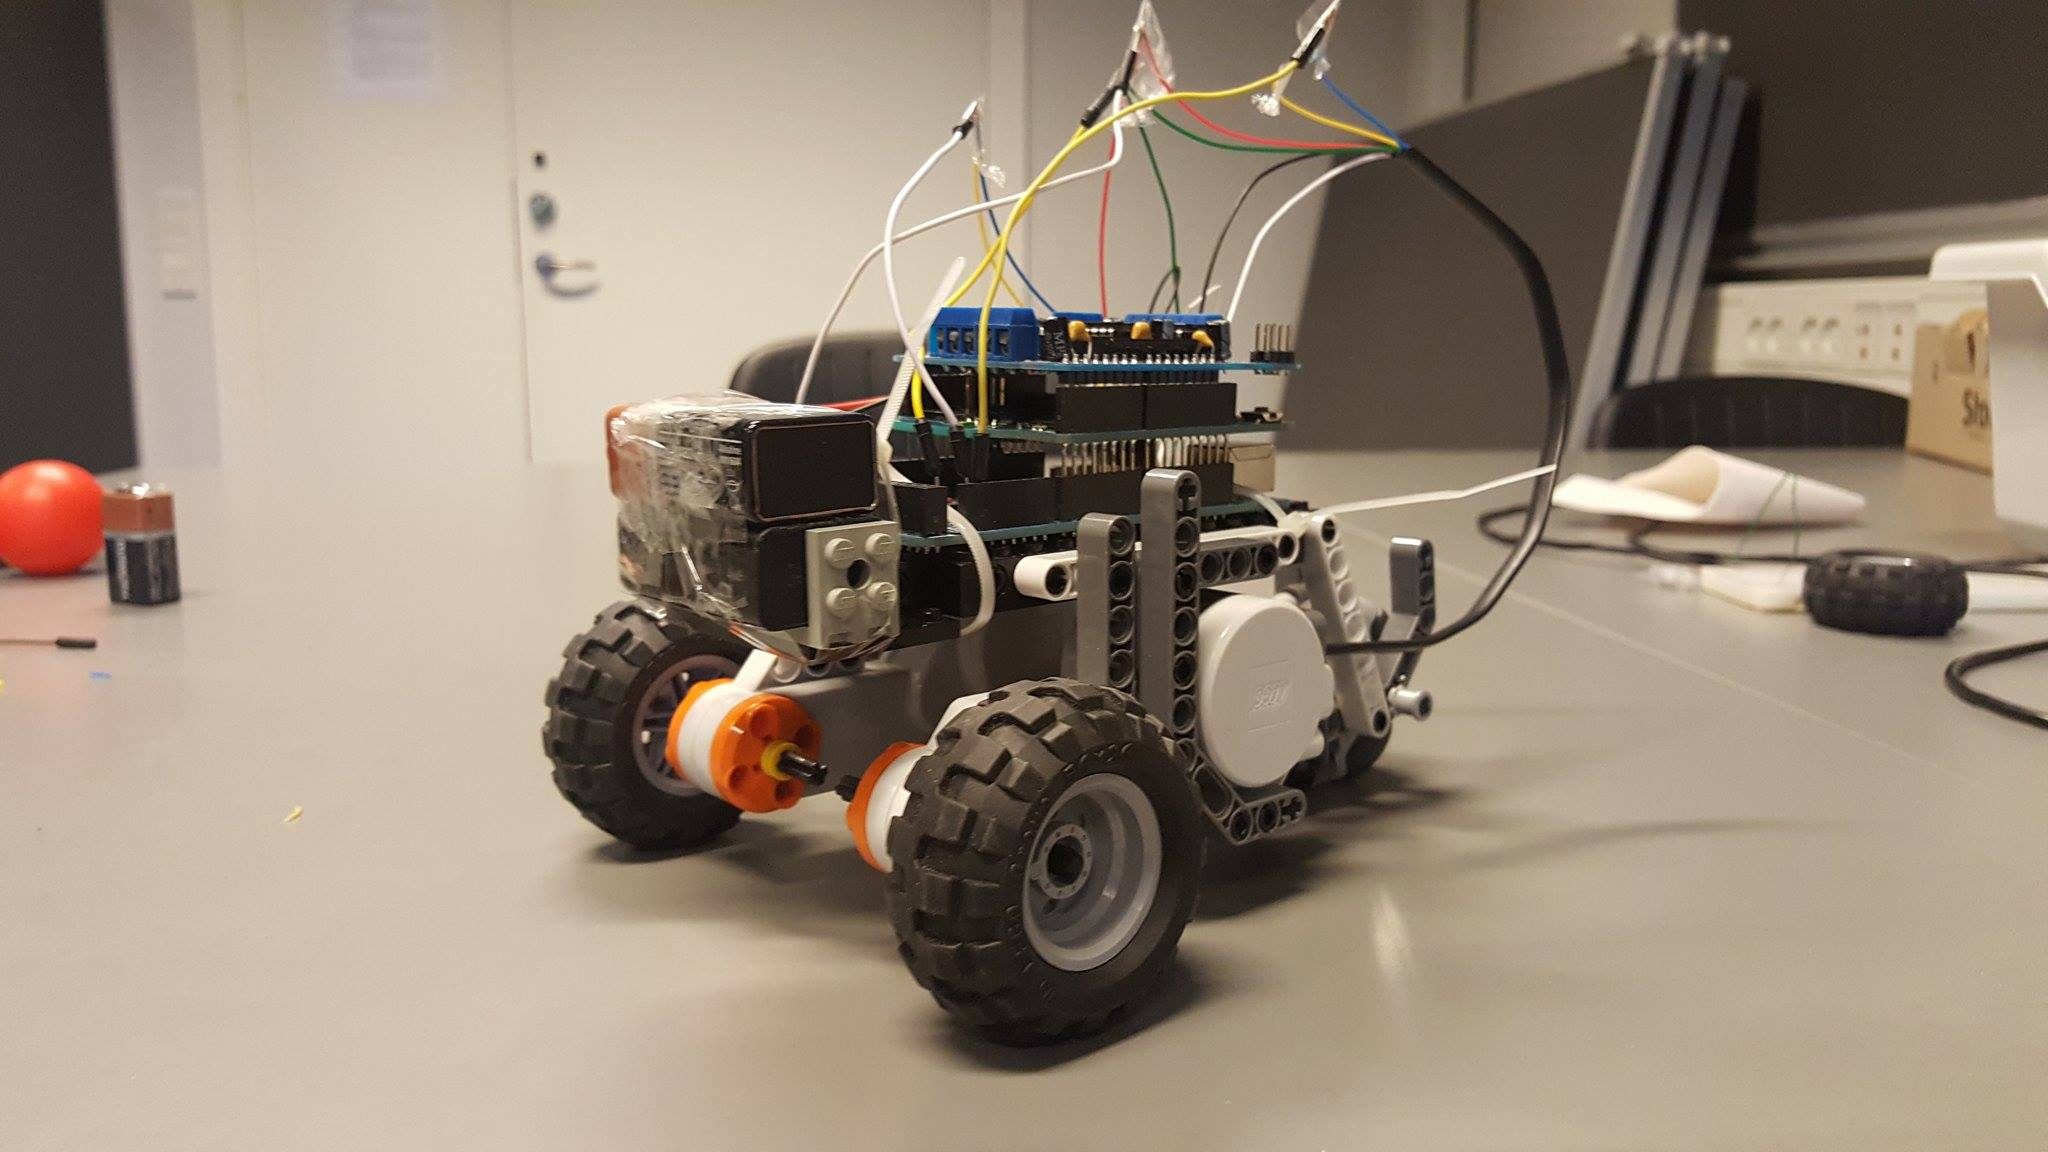
\includegraphics[scale=0.20]{billeder/robot}}
	\caption{The final design of the robot}
	\label{robot}
\end{figure}

The robot uses two LEGO NXT Servo motors with corresponding wheels, which will act as the front wheels. The back wheel can slide from side to side, which is important, since the wheel will be dragged sideways when the robots turns, a normal rubber wheel would have coursed a lot of friction. 
The robot are build around the NXT Servo motors, and ends with a platform at the top. This platform is for the Arduino and its shield to be stripped onto and for the batteries for the motor shield. 
The robot was build with  the arduino at the top, for easy access to the different pins if needed. 

\section{Arduino program design}
\label{sec:Arduino program design}
%Dette kan indeholde hvad vores program skal kunne gøre og evt. en punktform over hvilke funktioner/tasks som programmet løber i gennem.
As mentioned in section \ref{sec:Software choices}, the arduino program was developed in the Arduino IDE version 1.0.3. The program will be responsible to move the robot to the collision point, sent by the Kinect, of the object thrown at its predefined area. This is done by the program translating the coordinates from the Kinect, into coordinates know for the robot and move to that specific location

The program have a setup and will loop the behavior of the robot. First the sets up the WiFi connection to the Kinect program, it then waits for the Kinect program to send coordinates for the impact point of the object thrown. When it have received a set of coordinates, it will then translate the coordinates to so it knows where to move to. The next steps, the arduino program will continuously loop through until the program are exited: First it will check if it is at the impact point, if it is, the program is done. Else the robot will start moving, while it keeps adjusting it direction relative to the robots heading. Finally in the loop it will update the robots current position and its heading. All this can be broken down into tasks:

\begin{itemize}
	\item Make connection to the Kinect
	\item Wait to receive coordinates from the Kinect
	\item When the coordinates are received, it will translate these to useful coordinates and then enter the behavioral loop function:
	\begin{itemize}
		\item Check if already at the collision point, if it is exit program
		\item Start moving, adjust direction relative to heading
		\item Update the its position
	\end{itemize}
\end{itemize}
 

\section{Robot positioning and movement}
\label{sec:Robot positioning and movement}
%Kan indeholde hvordan vi har tænkt os med robottens kordinatsystem og hvordan den skal bevæge sig op i mod det punkt som den får fra kinecten.

\section{Connecting Arduino and Kinect}
\label{sec:Connecting Arduino and Kinect}
%Kan indeholde hvordan vi har tænkt os at de skal kunne snakke sammen og hvilket data der skal blive sendt i mellem dem.
For convenience, and as a part of the requirements for this project, the Arduino should receive wireless data from a computer, connected to the Kinect. The Arduino Wifi Shield makes this possible, with the Wifi library included in the Arduino IDE.
The connection between the Arduino and the computer should be through a local router, with a set SSID and password. The computer should use the Kinect to calculate an impact point of the object, and send this in a specific format, so that the data can be easily read and translated to a set of coordinates for the robots movement. The computer should be able to send coordinates more than once, since the first impact point is not necessarily be precise enough to catch the object. The computer should calculate increasingly accurate impact points, which should be sent with a certain minimal inter-arrival time, to not hinder the robots movement, and yet still in time for the robot to correct itself.
The Arduino should receive this data and read whenever it has sufficient time to do so, and convert the data received to match the right coordinate in the predefined area. 

\section{Scheduling}
\label{sec:Scheduling}
%Snakke om de forskellige tasks, deres deadlines og hvliken metode vi vil bruge til at schedule?
